\documentclass[11pt]{article}
\usepackage[includeheadfoot, top=1.0in, bottom=1.0in, hmargin=1.0in]{geometry}
\usepackage[utf8]{inputenc}
\usepackage{fancyhdr}
\pagestyle{fancy}
\usepackage{setspace}
\usepackage{tabularx}
\usepackage{xcolor}
\usepackage{cancel}
\usepackage{amsmath,amsfonts}
\usepackage{graphicx}
\usepackage{siunitx}
\usepackage{amssymb}

\usepackage[hyphens]{url}
\usepackage{hyperref}
\usepackage{enumitem}

\lhead{Astronomy Lab II}
\rhead{Spring 2022}
\lfoot{Mead \& Lee}
\rfoot{Mon 6-9pm}
\cfoot{\thepage}

\begin{document}

\begin{center}
\huge{Lab 9: Hubble's Law}\\ \medskip \Large{April 4, 2022}
\end{center}

\section{Introduction: The Expanding Universe}

\section{Hubble Trouble: Finding the Expansion Rate of the Universe}

\subsection{Retracing Hubble's steps}

\medskip \noindent
On CourseWorks (in the Lab 9 folder under ``Files''), open the spreadsheet titled ``hubble.xlsx''; the first tab (labeled ``1929'') shows Hubble's original data for 24 galaxies. Note that the velocity is labeled ``recession velocity'' -- this means that we're looking only at motions towards or away from us.  \textbf{Be sure to include the appropriate graphs in your lab write-up.}

\begin{enumerate}
    \item [3 pts] Make a scatter plot of Hubble's data, putting recession velocity (in km/s) on the vertical axis and distance (in Mpc) on the horizontal axis. For reference, 1 Mpc (``megaparsec'') is about 3 million light years, or about $3 \times 10^{19}$ kilometers.
    
    \begin{figure}[h!]
        \centering
        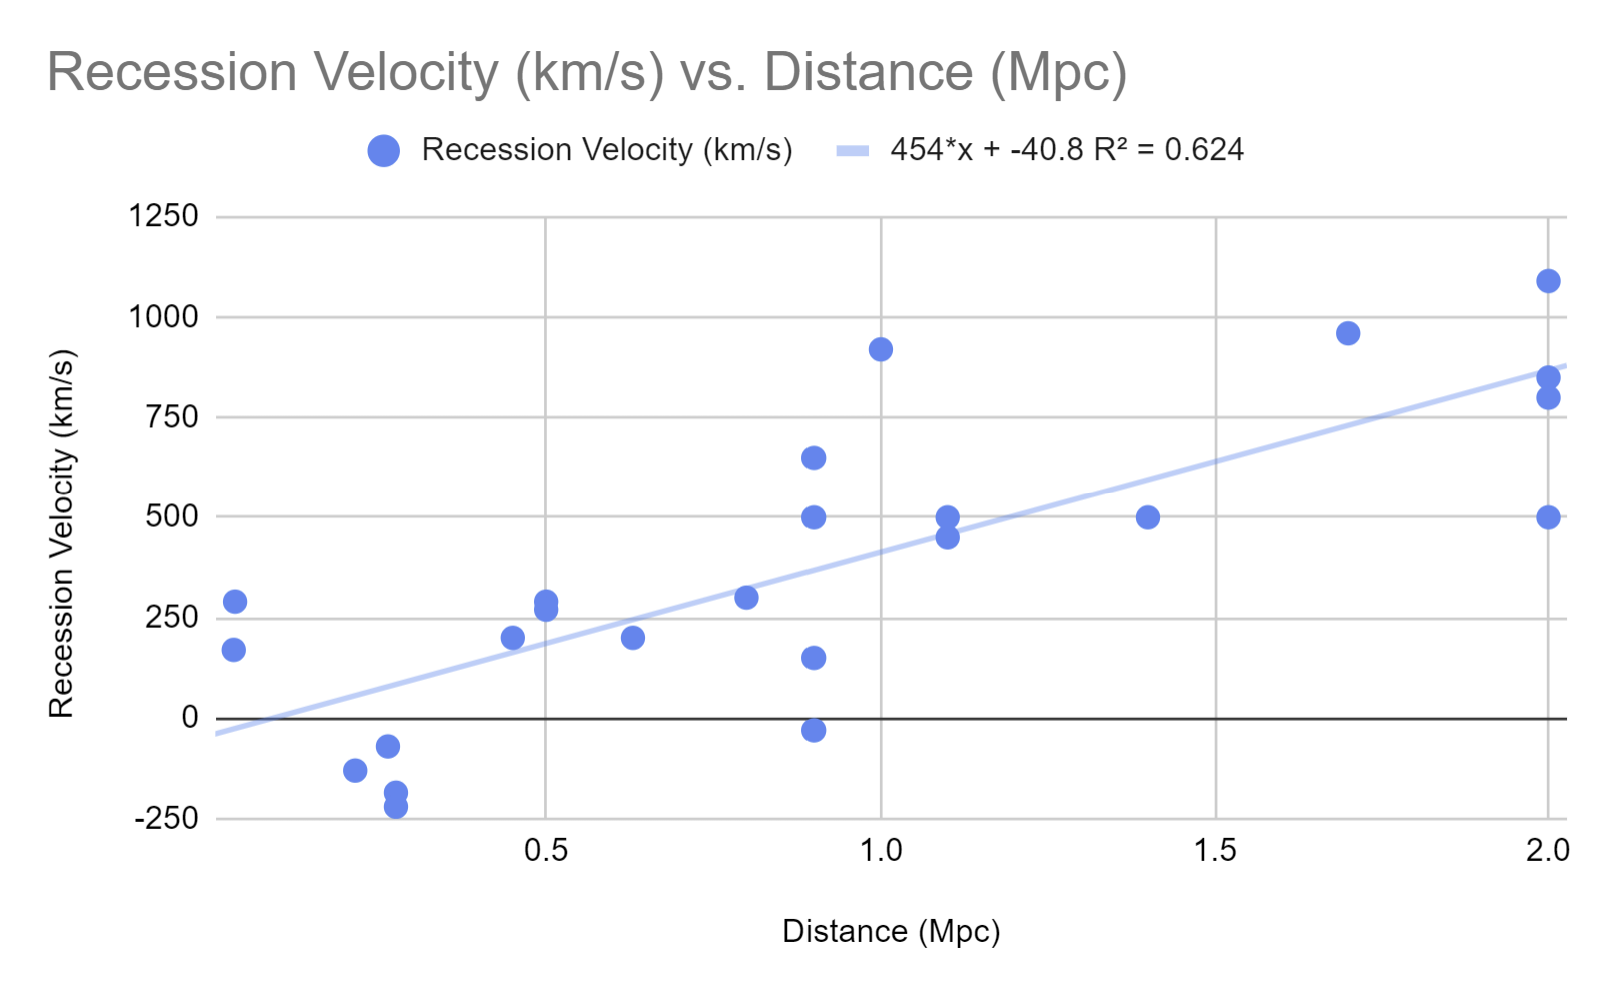
\includegraphics{Answer_Plots/Hubble 1929 Plot.png}
        \label{fig:1929}
    \end{figure}
    
    \item [10 pts] On the same figure, plot the line that best fits the data. In Google Sheets, you can do this by going to the ``Customize'' tab under the chart editor, clicking ``Series,'' and then checking the box labeled ``Trendline.'' 
        \begin{enumerate}
            \item Hubble's law predicts a linear trend between recession velocity and distance. How well does your trend line fit the data? Are you convinced that there's actually a linear trend in the data?
            
            \textcolor{red}{Vaguely linear, not well fit.  Lots of scatter, not convinced it's linear.}
            
            \item Why doesn't the line perfectly fit the data? That is, what are some sources of error or uncertainty that could be causing deviation from the predicted linear model?
            
            \textcolor{red}{Instrument/measurement error.  Cepheids not well calibrated.  Additional velocities (peculiar velocity if too close).}
            
            \item Does your line pass through the origin (i.e., does your line pass through the point of zero velocity and zero distance)? Do you expect the line to pass through the origin? (Hint: think about Equation \ref{eq:hubble})
            
            \textcolor{red}{It does not pass through the origin, but according to the equation, it should.}
            
            \item If your line doesn't pass through the origin, \emph{why} doesn't it?
            
            \textcolor{red}{Peculiar velocities cause deviations in nearby universe.}
        \end{enumerate}

    \item [10 pts] Slightly below the check box for ``Trendline,'' there's a drop-down menu for ``Label;'' set this to ``Use Equation,'' and enable the check-box labeled ``Show $R^2$'' below it.
        \begin{enumerate}
            \item For this best-fit line, what should be the \emph{units} of the slope? (Hint: remember that slope is ``rise over run,'' or the vertical change divided by the horizontal change)
            
            \textcolor{red}{km/s/Mpc}
            
            \item The equation of the best-fit line should be of the form $m \times x + b$, where $m$ is the slope and $b$ is the y-intercept. What is the slope of your best-fit line (remember to add units)? Congrats -- you've just measured the Hubble constant!
            
            \textcolor{red}{454 km/s/Mpc}
            
            \item What value do you get for $R^2$? $R^2$ is a measure of how good the line fits the data, with $R^2 = 1$ being a perfect fit. Would you characterize this linear model as a ``good'' fit?
            
            \textcolor{red}{$R^2=0.624$, not a great fit}
        \end{enumerate}

    \item [10 pts] Since the Hubble constant tells us how fast the Universe is (and has been) expanding, it also tells us how \emph{old} the Universe is. We can obtain a rough estimate for the age of the Universe by taking the reciprocal of the Hubble constant, or $1/H_0$.
    \begin{enumerate}
        \item The Hubble constant has weird units, so we'll first have to do some unit conversion. $1 \rm \, \frac{km/s}{Mpc} = 1.02 \times 10^{-12} \frac{1}{year}$. Use this to convert your measurement of $H_0$ to units of $\frac{1}{\rm year}$.
        
        \textcolor{red}{$4.63 \times 10^{-10} year^{-1}$}
        
        \item Now, compute $1/H_0$ to obtain the age of the Universe in years. Does your answer make sense?
        
        \textcolor{red}{$2.1 \times 10^9$ years or 2.1 Gyrs.  This is small.}
        
        \item Using radiometric dating of rocks, geologists have determined the age of the Earth to be about $4.5 \times 10^9$ years old. How does this compare to your estimate of the age of the Universe? Does this make sense?
        
        \textcolor{red}{This means the Earth is older than the Universe.  Kinda sus.}

       
    \end{enumerate}
\end{enumerate}

 \item [4 pts] The objects from Hubble's experiment are all local! $2\,\rm{Mpc}$ is very nearby and we expect objects this close to be gravitationally bound (one consequence of this is that gravity is opposing the expansion of the universe). How do you think this effects our estimate on the age of the universe? And what further data would you need to obtain a better estimate?

        \textcolor{red}{Local observations underpredict expansion because of the gravity pulling against bubble flow, need data from farther out}

\subsection{The limits of Hubble's law}

\begin{enumerate}
    \item [4 pts] Describe the trend in Figure \ref{fig:acceleration} at large distances (i.e., at large magnitude and redshift). Does the data still follow the linear trend predicted by Hubble's law?
    
    \textcolor{red}{At large distances, the data begins to curve away from the linear trend.}
    
    \item [4 pts] According to Hubble's law, objects that are more distant from us are receding from us faster, and thus the light emitted by more distant objects will be more redshifted. Light from more distant objects also takes longer to reach us, so more distant objects appear to be younger, or to have existed earlier in the Universe. In this sense, how can we use redshift as a proxy for cosmic time?
    
    \textcolor{red}{Higher redshift means light was emitted earlier in time. More distant light is more redshifted by expansion and also takes longer to reach the observer.}
    
    \item [4 pts] In Figure \ref{fig:acceleration}, a higher redshift corresponds to an object that existed earlier in the Universe; therefore, moving from high redshift to low redshift shows a progression from past to present. Given this, how has the Hubble constant (the slope of the best-fit line) evolved over time? Remember that the axes here are \emph{reversed} with respect to our previous plots!
    
    \textcolor{red}{The Hubble constant has gotten larger over time. The slope is shallower at higher redshift.}
\end{enumerate}

\begin{enumerate}[resume]
    \item [4 pts] Cosmologists believe that dark energy will forever remain dominant over matter. If this is the case, what will be the ultimate fate of the Universe?
    
    \textcolor{red}{The universe will expand forever.}
    
    \item [4 pts] If, somehow, matter were to become dominant over dark energy, how would this affect the ultimate fate of the Universe?
    
    \textcolor{red}{The universe would collapse.}
\end{enumerate}
20 pts

\section{A Stairway to Heaven: The Cosmic Distance Ladder}

\subsection{Parallax}

\medskip \noindent
Using Equation \ref{eq:parallax}, \textbf{answer the following questions in your lab write-up:}

\begin{enumerate}
    \item [3 pts] For an object at a fixed distance, how does $\theta$ change as you increase $B$? 
    
    \textcolor{red}{Theta increases as B increases.}
    
    \item [3 pts] For a fixed $B$, how does $\theta$ change as $D$ increases?
    
    \textcolor{red}{Theta decreases as D increases.}
\end{enumerate}

6 pts


\subsubsection{Parallax in Action: The Gaia Space Observatory}

\medskip \noindent
\textbf{Answer the following questions in your lab notebook:}

\begin{enumerate}[resume]
    \item [4 pts] Suppose you measure a parallax angle of $1''$ using a baseline of $B=2\;\mathrm{AU}$ ($1\;\mathrm{AU} \approx 1.496\times 10^{11}\;\mathrm{m} \approx 8\;\mathrm{light{-}minutes}$). Using Equation \ref{eq:parallax}, calculate the distance, $D$, to the object. Did you get something close to $206,265\;\mathrm{AU}$? This is how we define the \textbf{parsec} (or pc) -- the distance that produces a \emph{parallax of one (arc)second}.
    
    \textcolor{red}{206,265 AU}
    
    \item [10 pts] By using parsecs for distance ($D$) and arcseconds for the parallax angle ($\theta$), we can define a simpler relationship for parallax distance: $D = 1/\theta$. Using this formula and the fact that Gaia can measure parallaxes down to $20\;\mu\mathrm{as}$, what's the furthest distance Gaia can see? How does this distance compare to the distances you saw in Section 2? 
    
    \textcolor{red}{50000 pc, or 0.05 Mpc, a very small distance!}
\end{enumerate}

% \subsection{HR diagram fitting}
% Use NAAP labs thing. Students have already worked with HR diagrams, so they should be familiar with the main sequence and absolute/apparent magnitude (tho it may be helpful to redefine these terms  here).

\subsection{Cepheids}\label{sec:cepheids}

\textbf{Answer the following questions in your lab notebook}:

\begin{enumerate}
    \item [10 pts] A measured Cepheid has an apparent magnitude of 12 and a pulsation period of 10 days. 
    \begin{enumerate}
        \item Using the period-luminosity relationship given in Figure \ref{fig:cepheid_periodlum_relationship}, determine the absolute magnitude of the Cepheid. (reminder: magnitude measurements don't have units)
        
        \textcolor{red}{Absolute magnitude = -4 for a period of 10 days}
        
        \item Use the distance modulus (Equation \ref{eq:dm}) to determine the distance to this Cepheid variable (in parsecs).
        
        \textcolor{red}{$1.6 \times 10^4 pc$}
        
        \item Recall that a distance in parsecs (measured from the Earth) is related to a parallax angle in arcseconds via $D = 1/\theta$. What is the parallax angle of this Cepheid? Can we measure this parallax using Gaia?
        
        \textcolor{red}{$\theta = 0.000063$ arcseconds (63 $\mu$arcseconds) -- it can be measured by Gaia}
    \end{enumerate} 
    
    
    \item [4 pts] There are a number of steps/measurements involved in finding the distance to a Cepheid variable. What are some sources of error that could cause uncertainty in a Cepheid distance measurement? Recall that Edwin Hubble himself used Cepheid data in his 1929 paper.
    
    \textcolor{red}{Period/Luminosity may not be completely accurate, or there may be error in measuring either quantity.}
\end{enumerate}

\subsection{Supernova light curves}
%\textsl{Adapted from \href{http://physics.wm.edu/~labs/astro/}{William and Mary Introductory Astronomy (Physics 177) lab pages}}%

\medskip \noindent
The fourth tab of ``hubble.csv'' (the tab labeled ``NAAP SNIa'') lists 6 supernovae. For each of these supernovae, follow these instructions to fill out the spreadsheet.  \textbf{Make sure to include your completed spreadsheet and the appropriate graphs in your lab write-up.}

\begin{enumerate}
    \item [20 pts] Once you've fully filled out your spreadsheet, make a scatter plot of your supernova data with the recession velocity on the vertical axis and the distance on the horizontal axis. As you did in Section 2, fit a line to the data to find $H_0$. What value do you get for the Hubble constant?
    
    \textcolor{red}{Check they did this, and have reasonable $H_0$}
\end{enumerate}


\section{Conclusions}
\textbf{Answer the following questions in your lab write-up}:
\begin{enumerate}

    \item [4 pts] Qualitatively, what does Hubble's law tell us? What are the physical implications of Hubble's law?
    
    \textcolor{red}{Objects that are further away are receding from us faster.  This means the universe is expanding.}
    
    \item [10 pts] One big problem in modern cosmology (and one of the biggest problems in all of physics) is that \emph{we don't actually know} the correct value of $H_0$ -- measuring the expansion rate of the Universe in two different ways gives us two \emph{completely} different numbers. This problem is called the \textbf{Hubble tension}.
    \begin{enumerate}
        \item Read this short article describing the Hubble tension: \url{https://astrobites.org/2017/10/13/the-hubble-constants/}
        
        \item What are the two primary methods by which astronomers measure $H_0$, and what values of $H_0$ do each of these methods predict?
        
        \textcolor{red}{1) Supernovae + distance ladder (73.24 km/s/Mpc) 2) CMB (67.8 km/s/Mpc)}
        
        \item What might we learn by trying to understanding the source of the Hubble tension?
        
        \textcolor{red}{May learn new physics, improve understanding of early Universe.}
    \end{enumerate}

    \item Write down at least one question that you still have after finishing this lab.
    
    \item If you have any feedback on how today's lab was run, or if you have any suggestions for future lab sessions, please let me know!
    
    
\end{enumerate}
out of 125


\end{document}